\documentclass[11pt,a4paper]{report}

\ifx\pdftexversion\undefined
  \usepackage[dvips]{graphicx}
\else
  \usepackage[pdftex]{graphicx}
   \DeclareGraphicsRule{*}{mps}{*}{}
\fi

\usepackage{iftex}
\usepackage{color}
\ifPDFTeX
    \usepackage[utf8]{inputenc}
\fi
\usepackage[english]{babel}
\usepackage[english]{tuereport2008}
\usepackage{amsmath}
\usepackage{algorithm}
\usepackage{algpseudocode}
\usepackage[T1]{fontenc}
\usepackage{hyperref}
\usepackage{pgfplots}

\hypersetup{
    colorlinks,
    citecolor=black,
    filecolor=black,
    linkcolor=black,
    urlcolor=black
}

\graphicspath{{images/}}

\title{Visualizing the Netherlands}
\subtitle{2IV05: Additional component computer graphics}
\author{Michiel Fortuin\\Wouter Lok}
\version{2.0}
\orderissuer{}
\copyholder{}
\administrativeunit{Department of Mathematics and Computer Science}   % insert department name here
\department{Visualization}     % subdepartment, or group
\website{}
\reference{}

\begin{document}
\maketitle

\setcounter{tocdepth}{1}
\tableofcontents
\input{Changelog}
\chapter{Introduction}
This report presents the results of the project “Visualizing the Netherlands” as part of the course “Additional component computer graphics”. The goal of the project was to design and implement a system which is able to visualize the Netherland based on the BAG-extract [1] and other open data sources. The BAG-extract is a data set that contains information on all the buildings and addresses in the Netherlands.
%change reference

Firstly, the report presents the open data sets used, then the requirements and the desired functionality of the system is described. In section 4 the problems and challenges of the project are described shortly. Related work, which helped us solving the project’s challenges, is presented in section 5. In the literature study, methods to construct and visualize large worlds out of large data sets have been researched. Then in section 6, a short analysis of the used data sets is made and the system design and algorithms used are presented. The system uses specific data structures and methods to access the out-of-memory data set. Algorithms to construct and to use these data structures are also presented. Further, in section 7 the results of the implementation of the designed system and algorithms are discussed. Here the implemented system will be tested in various scenarios to see how the system performs. Finally a conclusion on the results is made and possible improvements or extensions on the systems are proposed.

\chapter{Problem description}
\label{chapter:ProblemDescription}
The main problem of this project is to build an interactive system that allows the real-time rendering of a large geographic data set in 3D. This goal gives rise to the following sub-problems:
\begin{itemize}
   \item Data from the geographic data set has to be processed and filtered
   \item Geographic models have to be generated from the process data
   \item The amount of memory and processing power available in common consumer computers is insufficient to hold and render all the models
\end{itemize}
Solutions to these problems are presented in section \ref{chap:AnalysisAndSolution}. 
\chapter{Open data sets}
The data required to render the Netherlands have been retrieved from two open data sets. Firstly, the BAG dataset [1] was used to extract all necessary information on buildings and secondly OpenStreetMap (OSM) [2] was used to retrieve information about the landscape.

The BAG (Basisadministratie Adressen en Gebouwen) is a data set which contains all kind of information on almost all the buildings and places in the Netherlands. The BAG is provided by Kadaster, but the content of the BAG is owned by the government of cities and they are also responsible to supply the information to Kadaster. A full extraction of the BAG data set called BAG-extract is freely available at various locations. We retrieved the dataset from the Nationaal georegister [3], a website which contains all kind of geographic open data sources. Our dataset contained a version from Januari 2014 and is 40 gB in total.

All information in the BAG-extract is supplied within xml-files and these files are grouped in multiple categories. Each category contains information on a different object-type. The different object-types are presented in table 1 and a full diagram containing all fields of the objects and connections between object types is presented in appendix 10.1. All geometric information in the BAG-extract is presented according to the Geography Markup Language (GML). GML is a standard format of providing geometric information with XML.

\begin{table}
    \begin{tabular}{cc}
      Object type & Content     \\
      Towns & Name, boundaries and status  \\
      Public spaces & Name of the place  \\
      Numbering & Addresses of buildings and places  \\
      Buildings & Building surface geometry, build year and status  \\
      Residences & Geometric location, surface area and status  \\
      Berths & Surface geometry and status  \\
      Other areas & Surface geometry and status \\
    \end{tabular}
    \caption{Object-types of the BAG-extract}
    \label{Table:ObjectTypesBAG}
\end{table}



\chapter{Requirements}
\label{chap:Requirements}
The application visualizes the Netherlands on the screen in 3D. All the buildings that are in the data set are being rendered. There are datasets for the whole of the Netherlands. It is possible to fly over an area of the Netherlands and walk through cities. Besides buildings, also roads and ground type (grass, farm land, water and industrial terrain) are rendered.
Because of the immensely huge data set of buildings in the BAG data set of the Netherlands, this data set has to be filtered, preprocessed and saved in an efficient format, so that it can be used by the algorithms to construct the world. OpenStreetMap has data about the streets, ground type and trees. That data set is also used to render the world.

\section{Specification of functionality}
\label{sec:SpecificationOfFunctionality}
The following functionality is implemented in the system.
\begin{itemize}
  \item Read data from the BAG data set.\\
    The BAG data set is quite large. The system needs to be able to read and filter the data from the BAG such that the required data can be retrieved.
  \item Construct buildings from geographic data. \\
    Models of buildings need to be constructed from the data read from the BAG. The model of a building has to be constructed to look like the corresponding real building.
  \item Construct roads and surface area.\\
    To make cities and other areas look like the real world, also roads and surface areas like grass, rivers and lakes can be constructed. These elements can contribute highly to make areas recognizable.
  \item Display the constructed world in 3D in real time.\\
    Since rendering a whole area, like Noord Brabant, can be quite large, an efficient rendering algorithm has to be designed and used so that the application can be rendered in real time.
\end{itemize}
\section{Specification of interaction}
\label{sec:SpecificationOfInteraction}
The user is able to use 3 different view modes. In the first view, the user is able fly through and over a city or a landscape and is able to freely control the direction of the movement. In the second view, the camera of the system will be set to a height around 1.75m and the user is not able to move vertically. That way, the user is able to see the world as any human would see it as he or she would walk through a city. Lastly, a top down view can be used in which the system shows the world like a map and the user is only able move horizontally and the user has the possibility to zoom in and out. To easily visit an other place, the user is able to select a city he or she would like to visit. The system then automatically travels somewhere above or within the city and then the user is again able to go anywhere her or she wants. Also the speed in which the user is walking or flying can be configured so that the user is able to walk quickly or slowly through the city or is able to quickly fly towards another city.

\section{Specification of presentation}
\label{sec:SpecificationOfPresentation}
In the world, buildings, roads, rivers, lakes and other types of surface areas are presented. For each type a different and appropriate texture is used, such that world is presented in such a way that it gives an impression of what the real world should look like. Also a sky is presented, such that the world gives even more an impression of a real world. 
\chapter{Discussion of literature}
Douglas Davis, William Ribarsky, T.Y. Jiang, Nickolas Faust and Sean Ho [6] present a method of rendering large collections of heterogeneous objects. By applying hierarchical paging procedures to terrain and buildings, they are able to visualize out-of-core collections of 3D objects (e.g. cities) in real-time.  Further they present the method efficient handling of culling on large collections of buildings. Finally, the use of levels of detail can be incorporated to provide detail management. This can be applied to solve the main part of the problem. 
\chapter{Analysis and solution}
\label{chap:AnalysisAndSolution}
\section{Data analysis}
\label{sec:DataAnalysis}
For each residence the BAG-dataset contains the surface area. In combination with the total area of the surface geometry of a building, the application approximates the amount of floors of a building. To approximate the height of a building, each floor is given the height of 2.5 meters.

Ways in OpenStreetMap contain tags. These tags can be used to determine what kind of way it is, for example the type of land, water, type of road. This information can be used to determine the texture which has to be applied. Furthermore, ways can contain meta-information.  For example, roads may contain information about the number of lanes of that road. This information is used to guess the width of the road. For every lane 2.5 meter is used.

\section{System Design}
\label{sec:SystemDesign}
The system is divided in three parts. The first part pre-processes all the data, to filter only data that is needed. For example it can filter only data that is in Eindhoven and remove any unneeded metadata. The second step is the Tree building application. The tree-builder uses the pre-processed data and generates the complete tree with all the models. The final part of the application uses the tree and the models to give visualization to the user.

\section{Algorithms}
\label{sec:Algorithms}
\subsection{HLOD}
\label{subsec:HLOD}
A way to render more data while still getting a good quality on screen, a quad tree data structure like the one used by Davis \cite{Davis} is used. The root of the tree is node that covers the complete dataset. A child of a node covers one quarter of the data set presented its parent.

A child node is created by geometrically splitting up the parent in four parts. This process is executed recursively until the triangle count of the data within the child node is below a specified threshold. The triangle count is the total number triangles needed to render all the models which are present within the node. When all the data models for all the children of a node have been generated, then this node will contain simplified versions of all the data models of its children.

Data models are simplified with the following algorithm. Of all the models within the node, the model which contains the two closest consecutive points is taken. These two closest consecutive points are average together to create one new point. This is done until the triangle count is below the specified threshold.

To addresses the problem what has to be rendered, the node manager is used. The node manager determines which nodes have to be loaded and rendered on screen. This is done by replacing nodes which is currently being used by its children or by its parent. We devised an algorithm that determines which node has to replace which node. By using tree traversal it finds all the maximal nodes which need to be loaded into main memory. This is done by checking whether the error assigned to a node as metadata meets the current distance to that node. If this node has to be loaded, and it isn’t loaded yet, it checks for its entire sub-tree which nodes are currently loaded. For every loaded node in its sub-tree it unloads the nodes. If the current node does not need to be loaded, while it is loaded it will also be unloaded. This way the node manager makes sure all the models will be loaded with the appropriate level of detail.

\subsection{Ear slicing algorithm}
\label{subsec:EarSlicingAlgorithm}
To produce the roof of a model, an ear slicing algorithm is used. Since most of the models of the buildings are non-convex polygons, not every point in the polygon is directly visible by all other points, and thus no direct edge can be constructed between two points without this edge crossing an edge of the polygon. The ear slicing algorithm is a well-known algorithm for triangulating a simple polygon \cite{Kajak11}. The algorithm iteratively locates an ear in the polygon and removes the ear. This process continues till the polygon is a triangle.

A vertex within a polygon is called an ear if the diagonal line between the neighbouring vertexes lies entirely within the polygon. That is, this diagonal does not intersect with any other edge of the polygon. When an ear is found, it is removed from the polygon and the diagonal will be a new edge within the polygon and the diagonal will be saved in a list. In the end, all the diagonals in the list form the triangulating diagonals for the polygon.

\subsection{Complex polygons}
\label{subsec:ComplexPolygons}
The OSM data is built out of GPS recordings and these recordings have a lot of noise. The noise has the possibility of creating complex polygons in the OSM data. A complex polygon is polygon that contains an self-intersecting edge. In our OSM data set we have detected multiple complex polygons. This is a problem because the ear-clipping algorithm can only be used for simple polygons. A simple polygon is a polygon that does not contain any self-intersecting edges. The detection for complex polygons is a naïve algorithm. If two non-consecutive line-segments intersect, then the polygon is complex.

To generate a set of simple polygons from a complex polygon, the algorithm has to find two line-segments that intersect. The point at which two edges intersect, two new polygons can be generated. These two new polygons can still be a complex polygon, so the algorithm has to be recursively called on these new polygons. If the input polygon is already simple, then it simply returns the input polygon.

\section{Motivation of choices made}
\label{sec:MotivationOfChoicesMade}
\subsection{Simple polygon test}
\label{subsec:SimplePolygonTest}
Testing if a polygon is simple is done in a naïve way, a faster method is for example the Bentley-Ottmann algorithm \cite{Bentley79}. This algorithm has a running time of $O(\frac{n^2}{\log{n}})$, which is faster that our naïve way with running time $O(n^2)$. We choose the naïve way, since the polygons in the data set are not very large. The largest polygon in the data set containing only Eindhoven had 60 points. Also the time in which we had to develop the application demanded that we used an algorithm that was relative simple to implement.

\subsection{Simple triangulation}
\label{subsec:SimpleTriangulation}
The ear slicing algorithm implemented also has a running time of $O(n^2)$. There also exist algorithms which can triangulate a polygon in $O(n\log(n))$ and $O(n)$ time. These algorithms are however also more complex to implement. And just like for the simple polygon test, our dataset only contains relatively small polygon, therefore longer running times do not form a great constraint.

\chapter{Results and evaluation}
\label{chap:ResultsAndEvaluation}
The results are created with the Netherlands data set. A detailed model of the Netherlands would be around 24.1 GB. This is too large to load in too GPU memory. The whole tree is around 55 GB in size. This tree consist about 2200 nodes of different sizes and has a depth around 12. The test PC has 8 GB of CPU memory and 1 GB of GPU memory.

\section{Image results}
\label{sec:ImageResults}
Figure \ref{fig:UniversityCampus} shows an overview of the TU/e campus. This is a basic view of the campus. The river dommel is also shown through the campus. This picture is taken above the train tracks.

\begin{figure}[htb!]
\centering
\includegraphics[width=\textwidth]{TUe}
\caption{University campus}
\label{fig:UniversityCampus}
\end{figure}

The error that is introduced when rendering from a distance is visible in figure \ref{fig:Simplification}. The top image is rendered with less error than the bottom version. In the simplified version, it is possible to see that the building is only a convex hull of its original. Also the roads that are besides the building are removed.

\begin{figure}[htb!]
\centering
\includegraphics[width=\textwidth]{Simplification}
\caption{Top: detailed version, Bottom: Simplified version}
\label{fig:Simplification}
\end{figure}

\section{GPU usage}
\label{sec:GPUUsage}
We have tested the system with 2 different error settings. The blue is with a 10 000 error per meter and a maximum error of 10 000 000. This means the largest distance loaded is 1 KM. The red is with a 100 000 error per meter and a maximum error of 1 000 000 000. This means the largest distance loaded is 10 KM.

In graph \ref{graph:MemoryUsage} we see that the memory usage for the blue error setting is far lower and not really dependent on the position. When red error setting is used the system is a bit more position dependent and uses a lot more memory, but can still be hold in the GPU memory. In graph \ref{graph:DistanceGraph} the distance is lower than the maximum distances for the specified setting. Note that this is the fartest node, but the closest distance to that node. Notice that the distance is almost 10 folded for both city's, while only doubling the memory usage.

\begin{figure}[htb!]
\centering
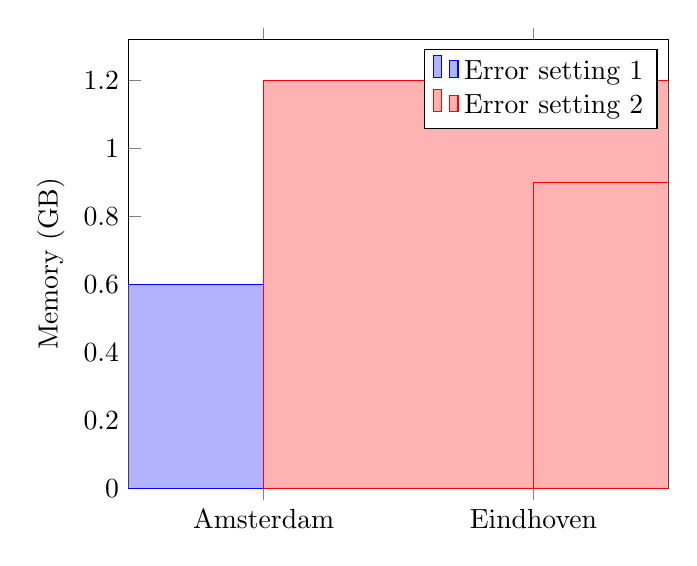
\begin{tikzpicture}
\begin{axis}[
    xtick={1,2},
    xticklabels={Amsterdam,
                Eindhoven},
    ybar=0pt,
    ymin=0,
    samples=2,
    domain=1:2,
    xtick=data,
    bar width=40,
    enlarge x limits={abs=0.5},
    ylabel={Memory (GB)}
]
        \addplot coordinates {
            (1,   0.6)
            (2,  0.6)
        };
        \addplot coordinates {
            (1,   1.2)
            (2,  0.9)
        };
        \legend{Error setting 1,Error setting 2}
\end{axis}
\end{tikzpicture}
\caption{Memory usage}
\label{graph:MemoryUsage}
\end{figure}

\begin{figure}[htb!]
\centering
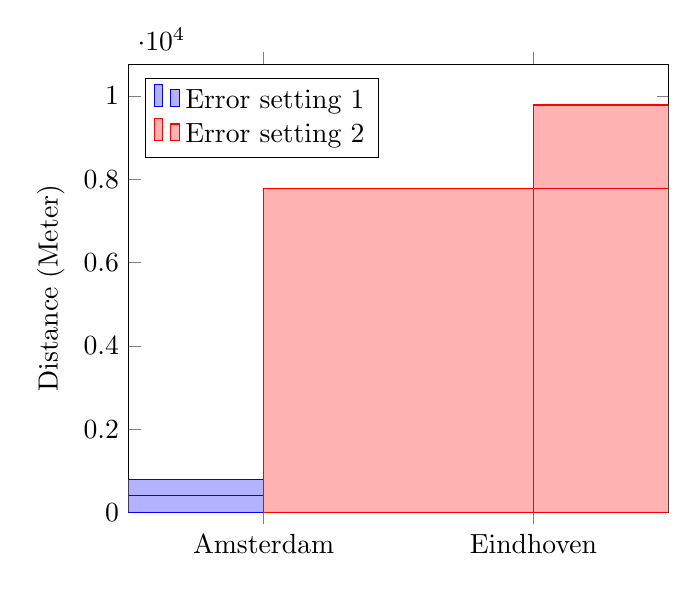
\begin{tikzpicture}
\begin{axis}[
    xtick={1,2},
    xticklabels={Amsterdam,
                Eindhoven},
    ybar=0pt,
    ymin=0,
    samples=2,
    domain=1:2,
    xtick=data,
    bar width=40,
    enlarge x limits={abs=0.5},
    ylabel={Distance (Meter)},
    legend pos=north west
]
        \addplot coordinates {
            (1,   407.557)
            (2,  797.977)
        };
        \addplot coordinates {
            (1,   7780.801)
            (2,  9786.661)
        };
        \legend{Error setting 1,Error setting 2}
\end{axis}
\end{tikzpicture}
\caption{Distance to furthest node}
\label{graph:DistanceGraph}
\end{figure}

\section{Limitations}
\label{sec:Limitations}
The height of buildings is determined with the building surface area of the building. If the building has an underground structure like underground parking garage, then the building is extremely high. The surface area of the geographic polygon is very small against the surface area of the whole building. This limitation expresses itself by generating very high building, while in reality the building above the ground is very low.

The width of a road is also approximated, by using meta-data. Sometimes this metadata isn’t available or wrong, which results in a different width. Also the road could have wider or smaller lanes.


\chapter{Conclusion and future work}
\label{chap:ConclusionAndFutureWork}
Our application can successfully render every building from Eindhoven, every element with grass and water and the roads. The objects have textures drawn on them to look appealing. Also different kinds of roads have different textures. The Buildings are generated from the BAG dataset and the other elements are generated from OpenStreetMap data set.

The data is rendered in real-time. Our tests show that a HLOD can make a big difference in rendering this kind of data. The GPU load is about 1.7 times lower with some error introduced, while the differences are not visible on the screen. The memory difference isn’t great. We assume that this is because the data set is relative small. Our single node data set is only 170MB. When the size increases, then the dataset does not fit in the GPU memory and then it will probably show that the memory usage is still very low.

The error that we introduce, which causes simplified versions of buildings to be rendered, is visible in some cases. This is only so little that most of the time this is unnoticeable. When there is a lot of occlusion then this error can even be increased, so the GPU has even less work.

The application can be improved by an algorithm that gives better result when simplifying the models. Also more data can be imported from OpenStreetMap. At the moment, all of our buildings have the same texture. The visualisation can be made even more appealing by applying different textures to buildings. This could be done based on the type of a building and the build year. Also more functionality could be introduced. Now, users can only fly or walk through the world to see what it looks like. The possibility to get information on buildings and the surrounding area would make the application more interesting.

\chapter{Bibliography}
\label{chap:Bibliography}
\begingroup
\renewcommand{\chapter}[2]{}% for other classes
\begin{thebibliography}{}
\bibitem{BAG14}
"BAG-Extract," Kadaster, [Online]. Available: http://www.kadaster.nl/web/artikel/productartikel/BAG-Extract.htm. [Accessed March 2014].
\bibitem{OSM14}
"Open Street Map," [Online]. Available: http://www.openstreetmap.org/about. [Accessed March 2014].
\bibitem{NG14}
"Inspire Adressen," [Online]. Available: http://geodata.nationaalgeoregister.nl/inspireadressen/atom{\slash}inspireadressen.xml. [Accessed February 2014].
\bibitem{NLExtract14}
"NLExtract," opengeogroep, [Online]. Available: https://github.com/opengeogroep/NLExtract. [Accessed February 2014].
\bibitem{OSMSharp14}
"OSMSharp," SharpSoftware, [Online]. Available: http://www.osmsharp.com/. [Accessed March 2014].
\bibitem{Davis}
D. Davis, W. Ribarsky, T. Jiang, N. Faust and a. S. Ho, "Real-Time Visualization of Scalably Large Collections of Heterogeneous Objects".
\bibitem{Kajak11}
B. Kajak, "Improved algorithms for ear-clipping triangulation," 2011.
\bibitem{Bentley79}
J. L. Bentley and T. A. Ottmann, "Algorithms for Reporting and Counting," IEEE TRANSACTIONS ON COMPUTERS,, Vols. c-28, no. 9, pp. 643-647, 1979.
\end{thebibliography}
\endgroup

\appendix
\chapter{Diagram structure BAG}
\label{chap:DiagramStructureBAG}
The diagram below presents the full data specification of the BAG-extract data set. It has been retrieved from the documentation provided by the Kadaster \cite{BAG14}.
\begin{figure}[htb!]
\centering
\includegraphics[width=\textwidth]{DiagramBAG.1}
\caption{Simple representation of the BAG-extract data set}
\label{fig:DiagramBAG}
\end{figure} 


\end{document} 